\chapter{La eficiencia de los algoritmos}

\section{El concepto de algoritmo}

Un algoritmo\footnote{La palabra \textit{algoritmo} proviene del nombre del matemático persa del siglo IX Abd Allah Muhhamad ibn Musa \textbf{al-Khwarizmi}.} es una \textit{secuencia finita ordenada de pasos exentos de ambigüedad tal que, al llevarse a cabo con fidelidad, dará como resultado la tarea para la que se ha diseñado}.
De esta definición podemos extraer algunos términos clave:

\begin{itemize}
	\item\textbf{Secuencia:} Los algoritmos se componen de instrucciones que deben realizarse una detrás de otra.
	\item\textbf{Finita:} Los algoritmos deben acabar en algún momento para poder producir un resultado.
	\item\textbf{Ordenada:} Las instrucciones que componen un algoritmo deben respetar un orden para desempeñar correctamente su tarea asociada.
	\item\textbf{Exentos de ambigüedad:} Los algoritmos no deben dejar ningún elemento a la libre interpretación del lector, ya que ésta cambiará su resultado.
	\item\textbf{Fidelidad:} Los algoritmos deben ser deterministas, es decir, deben producir el mismo resultado con la misma entrada.
\end{itemize}

Los algoritmos no son programas informáticos, aunque éstos pueden incorporar algoritmos para su correcto funcionamiento.
Los algoritmos deben cumplir necesariamente cinco propiedades:

\begin{itemize}
	\item\textbf{Ser nociones abstractas:} Los algoritmos no dependen del lenguaje en el que se implementen, sino que deben poder implementarse en varios lenguajes.
	\item\textbf{Estar bien definidos:} Cada paso de los algoritmos debe estar claramente expresado y sin ambigüedades.
	\item\textbf{Ser coherentes:} Los algoritmos deben producir el mismo resultado siempre que se le introduzcan los mismos datos iniciales.
	\item\textbf{Ser finitos:} Los algoritmos deben terminar.
	\item\textbf{Ser efectivos:} Los algoritmos deben resolver su problema asociado.
\end{itemize}

Un ejemplo de un mal algoritmo sería una receta de croquetas:

\begin{enumerate}
	\item $Echar\ aceite\ en\ la\ sartén$.
	\item $Esperar\ a\ que\ el\ aceite\ esté\ caliente$.
	\item $Echar\ croquetas\ en\ la\ sartén$.
	\item $Mientras\ las\ croquetas\ no\ se\ hayan\ dorado,\ esperar$.
	\item $Sacar\ las\ croquetas\ a\ un\ plato$:
\end{enumerate}

Aunque no cabe duda de que nos saldrían unas croquetas buenísimas siguiendo esta receta, falla como algoritmo por varios motivos.
Primero, no está \textbf{bien definido}.
¿Cuánto aceite echamos en la sartén?
¿Una garrafa?
¿Una pincelada?
¿Cuántas croquetas echamos en la sartén?
¿Qué nivel de dorado queremos que tengan las croquetas?
¿A qué potencia debemos poner el fuego?
¿En qué orden sacamos las croquetas?
Tampoco es \textbf{coherente}, ya que no siempre proporciona el mismo resultado.
En función del orden en que saquemos las croquetas algunas saldrán más hechas que otras en distintas iteraciones.
Por último, tampoco es \textbf{finito}.
Como no hemos especificado que ha de encenderse el fuego, ¡estaremos esperando eternamente a que el aceite esté caliente!

Siguiendo con analogías culinarias, esta receta de masa de pizza sí sería un buen algoritmo\footnote{Las medidas imperiales basadas en cucharas tienen equivalencias en el sistema métrico. Es una receta que sale muy rica.}:

\begin{enumerate}
	\item $Introducir\ 200g\ de\ agua\ a\ 20\ ^{\circ}C\ en\ la\ panificadora$.
	\item $Introducir\ 350g\ de\ harina\ de\ fuerza\ en\ la\ panificadora$.
	\item $Introducir\ una\ cucharada\ sopera\ de\ aceite\ en\ la\ panificadora$.
	\item $Introducir\ una\ cucharadita\ de\ sal$.
	\item $Introducir\ media\ cucharadita\ de\ azúcar\ moreno$.
	\item $Introducir\ 7\ gramos\ de\ levadura\ en\ polvo$.
	\item $Programar\ la\ panificadora\ para\ trabajar\ en\ modo\ \text{masa}\ durante\ 45\ minutos$.
	\item $Iniciar\ la\ panificadora$.
	\item $Esperar\ 45\ minutos$.
	\item $Extraer\ la\ masa\ de\ la\ panificadora$.
\end{enumerate}

En un ámbito más estrictamente matemático, éste también sería un ejemplo de un algoritmo correcto:

\begin{itemize}
	\item$a\leftarrow1$
	\item$i\leftarrow0$
	\item$Mientras\ (i<9)$, $hacer$:
	\begin{itemize}
		\item$a\leftarrow a\cdot2$
	\end{itemize}
	\item$Fin\ -\ Mientras$
	\item$Devolver(i)$
\end{itemize}

\section{La eficiencia de algoritmos: Problema, tamaño e instancia, principio de invarianza}

\subsection{Definiciones}

Dado un problema, podemos encontrar diferentes algoritmos que lo resuelven.
¿Cuál de todos es el mejor?
¿En qué situaciones podemos afirmar que uno es mejor que otro?
La eficiencia estudia la viabilidad de la implementación de un algoritmo para la resolución de un problema determinado.
Podemos medirla en función de los recursos que consume mediante dos factores:

\begin{itemize}
	\item\textbf{Tiempo:} Demora del algoritmo en la resolución del problema.
	\item\textbf{Espacio:} Recursos del sistema usados por el algoritmo.
\end{itemize}

A lo largo de esta asignatura nos centraremos en la dimensión temporal de la eficiencia.
Para estudiarla, debemos definir previamente cuatro conceptos:

\begin{itemize}
	\item\textbf{Problema:} Problema general a resolver expresado sin especificar unidades. Por ejemplo, ordenar ascendentemente un vector.
	\item\textbf{Instancia del problema:} Problema concreto derivado del problema general expresado con unidades. Por ejemplo, ordenar el vector \code{[3,5,1,2]}.

\pagebreak

	\item\textbf{Caso:} Conjunto de instancias con dificultad similar o idéntica
	\begin{itemize}
		\item\textbf{Caso peor:} Instancia en la que el algoritmo ejecuta el máximo de operaciones posible. Por ejemplo, ordenar ascendentemente por inserción un vector previamente ordenado descendentemente.
		\item\textbf{Caso promedio:} Instancia en la que tarda un tiempo medio. Se da generalmente cuando los datos iniciales son aleatorios.
		\item\textbf{Caso mejor:} Instancia en la que el algoritmo ejecuta el mínimo de posible. Por ejemplo, ordenar ascendentemente un vector previamente ordenado ascendentemente.
	\end{itemize}
	\item\textbf{Tamaño del caso:} tamaño de la instancia a resolver. Por ejemplo, el vector \code{[3,5,1,2]} es un caso de tamaño $n=4$.
\end{itemize}

Usaremos la notación $O(n)$ para indicar la eficiencia de un algoritmo en el caso peor y $\Omega(n)$ para su eficiencia en el caso mejor.
Ambos casos peor y mejor lo son únicamente para instancias del mismo tamaño.

Tomemos como ejemplo el siguiente algoritmo para ordenar un vector:

\begin{lstlisting}[language=C++]
void InsertionSort (double* v, int a, int b) {
	for (int i=a+1; i<=b; i++) {
		for (int j=i; j>a && v[j]<v[j-1]; j--) {
			double aux = v[j];

			v[j]   = v[j-1];
			v[j-1] = aux;
		}
	}
}
\end{lstlisting}

Este algoritmo ordena ascendentemente un vector \code{v} desde la posición \code{a} hasta la posición \code{b}, ambas inclusive.
Para ello, va comparando todos los valores desde la posición \code{a+1} hasta la posición \code{b} con el valor inmediatamente anterior a ellos (por ejemplo, cuando \code{i=1}, comparamos \code{a+1} con \code{a}) y lo intercambiamos con éste tantas veces como sea necesario hasta que el valor que estamos ordenando sea mayor que el anterior o esté en la primera posición a ordenar.
Éste es un caso de tamaño $n=a-b+1$ cuyo mejor caso es cuando \code{v} se introduce ordenado ascendentemente y cuyo peor caso es cuando \code{v} se introduce ordenado descendentemente.

A la hora de medir la eficiencia de un algoritmo podemos usar tres métodos:

\begin{itemize}
	\item\textbf{Método empírico:} Implementar el algoritmo y medir el tiempo de ejecución.
	\item\textbf{Método teórico:} Calcular una función que indique la evolución del algoritmo con respecto al tamaño del caso.
	\item\textbf{Método híbrido:} Una mezcla de ambos métodos.
\end{itemize}

\subsection{Principio de invarianza}

Al igual que un algoritmo debe ser independiente de un lenguaje, su eficiencia también lo es.
Llamamos a esta propiedad \textbf{Prinicpio de Inviarianza}:

\begin{displayquote}
\textit{Dadas dos implementaciones $I_1$ e $I_2$ de un mismo algoritmo, el tiempo de ejecución para una misma instancia de tamaño $n$, $T_{I_1}(n)$ y $T_{I_2}(n)$ no diferirá en más de una constante multiplicativa. Es decir, existe una constante positiva $K$ que verifica $T_{I_1}(n)\leq K\cdot T_{I_2}(n)$.}
\end{displayquote}

Teóricamente, esta constante $K$ es siempre igual para distintas ejecuciones del algoritmo, aunque en la práctica puede variar ligeramente debido a la carga del procesador a la hora de ejecutar el programa.
Lo que siembre será cierto es que, aunque dos lenguajes tarden tiempos diferentes en realizar la misma tarea, sus gráficas espacio-temporales tendrán la misma forma.
Por ejemplo, dos programas que ejecuten un algoritmo de eficiencia $O(n^2)$ en el peor caso mostrarán gráficas de curvatura $k\cdot n^2$.

\section{La notación asintótica, órdenes peor, mejor y exacto}

\subsection{Notación $\boldsymbol{O(f(n))}$}

Un algoritmo $A$ es de orden $O(f(n))$ para $f(n):\mathbb{N}\rightarrow\mathbb{R}^+$ si existe una implementación del mismo cuyo tiempo de ejecución $T_A(n)$ menor o igual que $K\cdot f(n)$ para una constante $K$ de casos de \textit{tamaño grande}.
Definido formalmente:

\[A\text{ es }O(f(n))\Leftrightarrow\exists K \in \mathbb{R}^+,\exists n_0\in\mathbb{N}:T_A(n)\leq K\cdot f(n)\forall n>n_0\]

Esta notación indica la eficiencia del algoritmo en el caso peor.
Se garantiza que el algoritmo nunca tardará más de $K\cdot f(n)$ unidades de tiempo en ejecutarse.
Existen varios órdenes de eficiencia, por ejemplo:

\begin{itemize}
	\item\textbf{Constante:} $O(1)$.
	\item\textbf{Lineal:} $O(n)$.
	\item\textbf{Cuadrático:} $O(n^2)$.
	\item\textbf{Logarítmico:} $O(\log(n))$.
	\item\textbf{Exponencial:} $O(a^n)$.
	\item\textbf{Factorial:} $O(n!)$.
\end{itemize}

Aunque para casos particulares puede ocurrir que un algoritmo sea más eficiente que otro a pesar de que su eficiencia teórica $O(n)$ sea peor (en el gráfico hay casos en los que $O(n)$ es mejor que $O(\log(n))$), siempre evaluaremos el algoritmo para un caso cuyo tamaño tiende a infinito.

\begin{center}
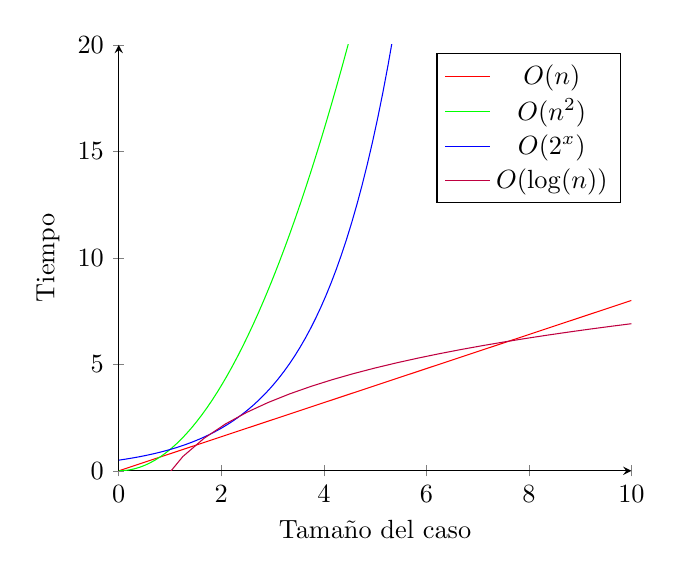
\begin{tikzpicture}[scale=0.95]
\begin{axis}[axis lines = left,
             xlabel = Tamaño del caso,
             ylabel = Tiempo,
				 ymin   = 0,
             ymax   = 20
            ]
\addplot[domain=0:10,
         samples=100,
         color=red
		  ]{0.8*x}; \addlegendentry{$O(n)$}
\addplot[domain=0:10,
         samples=100,
         color=green
		  ]{x^2}; \addlegendentry{$O(n^2)$};
\addplot[domain=0:10,
         samples=100,
         color=blue
		  ]{0.5*2^x}; \addlegendentry{$O(2^x)$};
\addplot[domain=0:10,
         color=purple
		  ]{3*ln(x)}; \addlegendentry{$O(\log(n))$};
\end{axis}
\end{tikzpicture}
\end{center}

Dados dos órdenes de eficiencia $O(f(n))$ y $O(g(n))$, podemos resolverlas calculando el límite al infinito de su cociente\footnote{Cálculo, tema 3.}:

\[\boldsymbol{O(f(n))\equiv O(g(n))}\Leftrightarrow\lim_{n\to\infty}\frac{f(n)}{g(n)}\rightarrow K\in\mathbb{R}^+\]
\[\boldsymbol{O(f(n))>O(g(n))}\Leftrightarrow\lim_{n\to\infty}\frac{f(n)}{g(n)}\rightarrow\infty\]
\[\boldsymbol{O(f(n))<O(g(n))}\Leftrightarrow\lim_{n\to\infty}\frac{f(n)}{g(n)}\rightarrow0\]

Tomemos como ejemplo un algoritmo $A$: $O(n^2)$ y un algoritmo $B$: $O({(4n+1)}^2+n)$:

\[\lim_{n\to\infty}\frac{f(n)}{g(n)}=\lim_{n\to\infty}\frac{n^2}{{(4n+1)}^2+n}=\lim_{n\to\infty}\frac{n^2}{16n^2+9n+1}=\lim_{n\to\infty}\frac{1}{16}\]

Ambos algoritmos son de eficiencia equivalente y nos referimos a ellos como algoritmos de eficiencia $O(n^2)$ para simplificar.
Tomemos ahora un algoritmo $A$: $O(n)$ y un algoritmo $B$: $O(n\cdot\log(n))$:

\[\lim_{n\to\infty}\frac{f(n)}{g(n)}=\lim_{n\to\infty}\frac{n}{n\cdot\log{n}}=\lim_{n\to\infty}\frac{1}{\log(n)}=0\]

El algoritmo $A$ es más eficiente que $B$.
Como último ejemplo, tomemos un algoritmo $A$: $O({(n^2+29)}^2)$ y un algoritmo $B$: $O(n^3)$:

\[\lim_{n\to\infty}\frac{f(n)}{g(n)}=\lim_{n\to\infty}\frac{{(n^2+29)}^2}{n^3}=\infty\]

Existen problemas cuyo tamaño depende de más de una variable, en cuyo caso se analiza el caso considerando que la aridad de la función $f$ es tan alta como el número de variables.

\[A\text{ es }O(f(n,m))\Leftrightarrow\exists K\in\mathbb{R}^+:T_A(n,m)\leq K\cdot f(n,m)\forall n,m\]

\subsection{Notación $\boldsymbol{\Omega(f(n))}$}

Un algoritmo $A$ es de orden $\Omega(f(n))$ para $f(n):\mathbb{N}\rightarrow\mathbb{R}^+$ si existe una implementación del mismo cuyo tiempo de ejecución $T_A(n)$ es mayor o igual que $K\cdot f(n)$ para una constante $K$ de casos de \textit{tamaño grande}.
Definido formalmente:

\[A\text{ es }\Omega(f(n))\Leftrightarrow\exists K\in\mathbb{R}^+,\exists n_0\in\mathbb{N}:T_A(n)\geq K\cdot f(n)\forall n>n_0\]

Se garantiza que el algoritmo nunca tardará menos de $K\cdot f(n)$ unidades de tiempo en ejecutarse.
La constante $K$ de las notaciones $O$ y $\Omega$ toma valores individuales en cada caso que podrían ser iguales.

\subsection{Notación $\boldsymbol{\Theta(f(n))}$}

Un algoritmo $A$ es de orden exacto $\Theta(f(n))$ para $f(n):\mathbb{N}\rightarrow\mathbb{R}^+$ cuando el tiempo de ejecución del algoritmo puede expresarse siempre commo $T_A(n)=K\cdot f(n)$, en cuyo caso dicho algoritmo es simultáneamente de orden $O(f(n))$ y $\Omega(f(n))$.
Definido formalmente:
\[A\text{ es }\Theta(f(n))\Leftrightarrow\exists K\in\mathbb{R}^+,\exists n_0\in\mathbb{N}:T_A(n)=K\cdot f(n)\forall n\]

\subsection{Propiedades y reglas de los órdenes de eficiencia}

Los órdenes de eficiencia cumplen las siguientes propiedades:

\begin{itemize}
	\item\textbf{Transitiva:} $f(n)\in O(g(n))\land g(n)\in O(h(n))\Rightarrow f(n)\in O(h(n))$.
	\item\textbf{Reflexiva:} $f(n)\in O(f(n))$.
	\item\textbf{Simétrica:} $f(n)\in\Theta(g(n))\Leftrightarrow g(n)\in\Theta(f(n))$.
	\item\textbf{Suma de órdenes:} $T_1(n)\in O(f(n))\land T_2(n)\in O(g(n))\Rightarrow T_1(n)+T_2(n)\in O(\max(f(n),g(n)))$.
	\item\textbf{Producto de órdenes:} $T_1(n)\in O(f(n))\land T_2(n)\in O(g(n))\Rightarrow T_1(n)\cdot T_2(n)\in O(f(n)\cdot g(n))$.
\end{itemize}

Las propiedades transitiva y reflexiva también se cumplen para $\Omega$ y $\Theta$.
De estas propiedades podemos extraer tres reglas:

\begin{itemize}
		  \item\textbf{Regla del máximo:} $O(f(n)+g(n))=\max(O(f(n)),O(g(n)))$.
		  \item\textbf{Regla de la suma:} $O(f(n)+g(n))=O(f(n))+O(g(n))$.
		  \item\textbf{Regla del producto:} $O(f(n)\cdot g(n))=O(f(n))\cdot O(g(n))$.
\end{itemize}

\section{Análisis de algoritmos}

Analizar la eficiencia teórica $O(f(n))$ de un algoritmo requiere, como primer paso, detectar las variables de las que depende su tamaño.
Hecho esto, vamos analizando cada uno de los pasos, que pueden presentar diferentes tipos de sentencias.

\subsection{Operaciones elementales}

Son aquellas cuya ejecución no depende del tamaño del caso, ya que su tiempo máximo está acotado.
Debido a esta acotación, su orden de eficiencia en el caso peor es $O(1)$.
Es el caso de operaciones sobre tipos primitivos, apertura de ficheros, declaración de variables, entrada o salida de datos y otras operaciones que no trabajan con estructuras de tamaño variable.

\begin{lstlisting}[language=C++]
int x = 0;
x = x+8;
printf("El valor de x ahora es %d\n", x);
std::ofstream fo;
fo.open("salida.log");
\end{lstlisting}

\subsection{Sentencias condicionales}\label{condicionales}

Son aquellas que se componen de la evaluación de una condición y la ejecución de un bloque en función del resultado de dicha condición:

\begin{lstlisting}[language=C]
if (!(x%2)) {   // Condición
	x /= 2;      // Bloque 1
}
else {
	x = (x*3)+1  // Bloque 2
}
\end{lstlisting}

El tiempo de ejecución de las sentencias condicionales está acotado tanto en el caso mejor como en el caso peor:

\[O(f(n))=\max\big(O(Condici\acute{ó}n),O(Bloque_1),O(Bloque_2)\big)\]
\[\Omega(f(n))=\Omega(Condici\acute{o}n)+\min\big(O(Bloque_1),O(Bloque_2)\big)\]

\subsection{Sentencias repetitivas}\label{repetitivas}

Son aquellas que se componen de una condición y un bloque de sentencias que se ejecuta si se cumple dicha condición y hasta que ésta deje de cumplirse.

\begin{lstlisting}[language=C]
while (x<10) { // Condición
	x += 1;     // Bloque
}
\end{lstlisting}

Para una sentencia con una condición de eficiencia $c(n)$ y un bloque de eficiencia $b(n)$ que se ejecute $f(n)$ veces, la eficiencia de dicha sentencia será la siguiente:

\[O\Big(c(n)+f(n)\cdot\big(b(n)+c(n)\big)\Big)\]

Esto se debe a que primero evaluamos la condición ($c(n)$) y luego ejecutamos $f(n)$ veces el bucle, que ejecuta el bloque y luego la condición ($b(n)+c(n)$) en cada iteración hasta finalizar.

Como caso particular del bucle \code{while}, tenemos el bucle \code{do while}:

\begin{lstlisting}[language=C]
do {
	x += 1;      // Bloque
} while (x<10); // Condición
\end{lstlisting}

Su orden de eficiencia, que debe tener en cuenta que el bloque se ejecuta siempre al menos una vez, es el siguiente:

\[O\Big(b(n)+c(n)+f(n)\cdot\big(b(n)+c(n)\big)\Big)\]

Por último, tenemos el caso del bucle \code{for}:

\begin{lstlisting}[language=C]
for (int i=0; i<vector.size(); i++) { // Inicialización; Condición; Actualización
	vector[i] = 0;                     // Bloque
}
\end{lstlisting}

Para un bucle con una inicialización de eficiencia $i(n)$, una condición de eficiencia $c(n)$, una actualización de eficiencia $a(n)$ y un bloque de eficiencia $b(n)$ que se ejecuta $f(n)$ veces, la eficiencia de dicho bucle será la siguiente:

\[O\Big(i(n)+c(n)+f(n)\cdot\big(b(n)+a(n)+c(n)\big)\Big)\]

A continuación se muestran como ejemplo el cálculo de la eficiencia de un bucle \code{while} y un bucle \code{for}:

\begin{lstlisting}[language=C]
int main (int argc, char** argv) {
	int n = atoi(argv[1]);

	while (n>0) {
		for (int i=0; i<n; i*=2) {
			printf("%d, ", i);
		}
		printf("\n");
		n--;
	}
}
\end{lstlisting}

Fijémonos primero en el interior del bucle \code{for}.
La eficiencia de la llamada a \code{printf} es siempre $O(1)$, al igual que lo son su inicialización, condición y actualización.
El bucle se ejecuta de $i$ a $n$ en saltos de $2i$, por lo que se ejecutará siempre $\log_2(i)$ veces.
El orden de eficiencia del bucle for es $O\big(\log(n)\big)$.
Resulelto esto, calculamos la eficiencia del bloque del bucle \code{while}.
Como las otras dos sentencias son de orden de eficiencia $O(1)$, la eficiencia del bloque del bucle \code{while} es $O\big(\log(n)\big)+2\cdot O(1)=O\big(\log(n)\big)$.
Por último, la condición del bucle while es una sentencia se orden de eficiencia $O(1)$ y este bucle se ejecuta $n$ veces, por lo que la eficiencia total de este bucle es $O\big(n\cdot\log(n)\big)$.

\pagebreak

\subsection{Secuencias de sentencias}\label{secuenciasentencias}

Cuando un algoritmo ejecuta secuencialmente varios bloques de sentencias $S_i$ con órdenes de eficiencia $O\big(f_i(n)\big)$, aplicamos las reglas de la suma y el máximo para calcular la eficiencia total:

\[O\Big(\sum_{i=0}^{k}f_k(n)\Big) = \max\Big(O\big(f_0(n)\big),O\big(f_1(n)\big),\ldots,O\big(f_{n-1}(n)\big)\Big)\]

Por ejemplo, el programa mostrado en~\ref{repetitivas} contiene una asignación de orden de eficiencia $O(1)$ y un bucle de orden de eficiencia $O\big(n\cdot\log(n)\big)$, por lo que la eficiencia total del programa es $O\big(n\cdot\log(n)\big)$.

\subsection{Llamadas a funciones no recursivas}

La eficiencia de una llamada a una función depende de si sus argumentos de entrada dependen o no del tamaño del problema.
Tomemos como ejemplo la siguiente función que calcula si un número es primo:

\begin{lstlisting}[language=C]
bool EsPrimo (unsigned num) {
	bool primo = false;
	unsigned max = sqrt(num);

	for (unsigned i=2; i<=max && !primo; i++) {
		primo = !(valor%i);
	}

	return primo;
}
\end{lstlisting}

El bucle \code{for} tiene un orden de eficiencia de $O(n)$ (en el caso peor itera hasta \code{i<=max}), pero \code{max} se calcula como \code{sqrt(num)}, por lo que la eficiencia del algorimo es $O(\surd n)$.
Veamos cuatro ejemplos de bucles que incorporan una llamada a \code{EsPrimo()} y sus respectivas eficiencias:

\begin{lstlisting}[language=C]
for (unsigned i=0; i<n; i++) {
	if (EsPrimo(1337))
		printf(%d, ", i);
}
\end{lstlisting}

Este algoritmo tiene eficiencia $O(n)$, ya que la llamada \code{EsPrimo(1337)} no varía en el función del caso y se ejecuta en tiempo constante.

\begin{lstlisting}[language=C]
for (unsigned i=0; i<n; i++) {
	if (EsPrimo(i))
		printf(%d, ", i);
}
\end{lstlisting}

Este algoritmo tiene eficiencia $O(n\cdot\surd n)$, ya que aquí la eficiencia de llamada a \code{EsPrimo(i)} sí depende del tamaño del caso.

\begin{lstlisting}[language=C]
for (unsigned i=0; i<2000; i++) {
	if (EsPrimo(i))
		printf(%d, ", i);
}
\end{lstlisting}

Este algoritmo tiene eficiencia $O(1)$, ya que siempre se va a ejecutar $2000$ veces y va a calcular \code{EsPrimo(i)} de los mismos $2000$ valores.

\pagebreak

\begin{lstlisting}[language=C]
for (unsigned i=n; i>0; i/=2) {
	if (EsPrimo(i))
		printf(%d, ", i);
}
\end{lstlisting}

Por último, este algoritmo tiene eficiencia $O\big(\log(n)\cdot\surd n\big)$, ya que el bucle \code{for} ejecuta $\log_2(n)$ veces una llamada de eficiencia $O(\surd n)$.

\subsection{Llamadas a funciones recursivas}

\section{Resolución de recurrencias}
